\section*{Section \ref{S:setoperations} Sets and Set Operations}

\begin{enumerate}
\item \begin{tabular}[t]{p{1.2in} p{1.2in} p{1.2in}}
(a) $A = B$  &  (c) $C \ne D$  &  (e) $A \not \subseteq D$ \\
(b) $A \subseteq B$  &  (d) $C \subseteq D$ &  \\
\end{tabular}


\item In both cases, the two sets have precisely the same elements.  The order in which the elements are written is not important, and it makes no difference how many times a certain element is repeated in the list.


\item \begin{tabular}[t]{r c l c r c l }
$A$ & $\subset, \subseteq , \ne$ & $B$ &  &  $\emptyset$ & $\subset , \subseteq , \ne$ & $A$  \\
5   & $\in$ & $C$ & & $\left\{ 5 \right\}$ & $\subset , \subseteq , \ne$ & $C$ \\
$A$ & $\subset, \subseteq , \ne$ & $C$ &  &  $\left\{ 1,2 \right\}$ & $\subset, \subseteq , \ne$ & $B$ \\
$\left\{ 1,2 \right\}$ & $\ne$ & $A$ &  &  $\left\{ 3,2,1 \right\}$ & $\subset, \subseteq , \ne$ & $D$ \\
4  &  $\notin$ &  $B$ &  &  $D$ &  $\ne$ &  $\emptyset$ \\
$\left| A \right|$ &  $=$ & $\left| D \right|$ & & $\left| A \right|$ & $\ne$ & $\left| B \right|$ \\
$A$ & $\in$ &  $\mathcal{P} \left( A \right)$ & & $A$ & $\in$ &  $\mathcal{P} \left( B \right)$ \\
\end{tabular}


\item \begin{tabular}[t]{l l l}
$\mathbb{N} \subset \mathbb{Z}$  &  $\mathbb{N} \subset \mathbb{Q}$ & 
$\mathbb{N} \subset \mathbb{R}$   \\
$\mathbb{Z} \subset \mathbb{Q}$  &  $\mathbb{Z} \subset \mathbb{R}$   & $\mathbb{Q} \subset \mathbb{R}$ \\
\end{tabular}


\item \begin{enumerate}
\item The set $\left\{ {a, b} \right\}$ is a not a subset of  $\left\{ {a, c, d, e} \right\}$
 since  $b \in \left\{ {a, b} \right\}$ and  $b \notin \left\{ {a, c, d, e} \right\}$.

\item $\left\{ { - 2,0,2} \right\} = \left\{ {x \in \mathbb{Z} \mid  
x\text{ is even  and  }x^2  < 5} \right\}$ since both sets have precisely the same elements.

\item $\emptyset \subseteq \left\{ 1 \right\}$ since the following statement is true:
For every $x \in U$, if $x \in \emptyset$, then $x \in \left\{ 1 \right\}$.

\item The statement is false.  The set $\left\{ a \right\}$ is an element of 
$\mathcal{P} \left( A \right)$.
\end{enumerate}


\item \begin{enumerate}
\item $x \notin A \cap B$ if and only if $x \notin A$ or $x \notin B$.

\item $x \notin A \cup B$ if and only if $x \notin A$ and $x \notin B$.

\item $x \notin A - B$ if and only if $x \notin A$ or $x \in B$
\end{enumerate}



\item \begin{multicols}{2}
\begin{enumerate}
  \item $A \cap B = \left\{ 5, 7 \right\}$
  \item $A \cup B = \left\{ 1, 3, 4, 5, 6, 7, 9 \right\}$
  \item $\left( {A \cup B} \right)^c = \left\{ 2, 8, 10 \right\}$
  \item $A^c  \cap B^c = \left\{ 2, 8, 10 \right\}$
  \item $( {A \cup B} ) \cap C = \left\{ {3, 6, 9} \right\}$
  \item $A \cap C = \left\{ 3, 6 \right\}$
  \item $B \cap C = \left\{ 9 \right\}$
  \item $( {A \cap C} ) \cup ( {B \cap C} ) = \left\{ 3, 6, 9 \right\}$
  \item $B \cap D = \emptyset$
  \item $\left( {B \cap D} \right)^c = U$
  \item $A - D = \left\{ 3, 5, 7 \right\}$
  \item $B - D = \left\{ 1, 5, 7, 9 \right\}$
\end{enumerate}
\end{multicols}
\begin{enumerate} \setcounter{enumii}{12}
  \item $\left( {A - D} \right) \cup \left( {B - D} \right) = \left\{ 1, 3, 5, 7, 9 \right\}$
  \item $\left( {A \cup B} \right) - D = \left\{ 1, 3, 5, 7, 9 \right\}$
\end{enumerate}


\item \begin{enumerate}
\item $A \cap B = \{7, 9, 11, 13, \ldots \, \}$

\item $A \cup B = \{1, 3, 5, 7, 8, 9, 10, 11, \ldots \, \}$

\item $(A \cup B)^c = \{2, 4, 6 \}$

\item $A^c \cap B^c = \{2, 4, 6 \}$

\item $( {A \cup B} ) \cap C = \{3, 9, 12, 15, 18, \ldots \, \}$

\item $( {A \cap C} ) \cup ( {B \cap C} ) = \{3, 9, 12, 15, 18, \ldots \, \}$

\item $B \cap D = \emptyset$

\item $(B \cap D)^c = \N$

\item $A - D = \{7, 9, 11, 13, \ldots \, \}$

\item $B - D = \{1, 3, 5, 7, 9, \ldots \, \}$

\item $(A - D) \cup (B - D) = \{1, 3, 5, 7, 9, \ldots \, \}$

\item $(A \cup B) - D = \{1, 3, 5, 7, 9, \ldots \, \}$
\end{enumerate}





\item \begin{enumerate}
\item For each $x \in U$, if $x \in \left( P - Q \right)$, then $x \in R \cap S$.

\item There exists an $x \in U$ such that $x \in \left( P - Q \right)$ and $x \notin R \cap S$.

\item For each $x \in U$, if $x \notin R \cap S$, then $x \notin \left( P - Q \right)$.
\end{enumerate}



\item If $A \subseteq B$, then $B^c \subseteq A^c$.
\begin{enumerate}
\item One conditional statement is the given statement.  The hypothesis can be written as a conditional statement as follows:  If $x \in A$, then $x \in B$.  The conclusion can be written as a conditional statement as follows:  If $y \in B^c$, then $y \in A^c$.

\item The contrapositive is:  For all $A$, $B$, and $C$ that are subsets of $U$, if $B^c \not \subseteq A^c$, then $A \not \subseteq B$.

\item The negation is:   There exist $A$, $B$, and $C$ that are subsets of $U$ such that $A \subseteq B$ and $B^c \not \subseteq A^c$.



%\item $\left( \forall A,B \in \mathcal{P} \left( U \right) \right) \left[ \left( A \subseteq B \right) \to \left( B^c \subseteq A^c \right) \right]$
%
%\item $\left( \exists A,B \in \mathcal{P} \left( U \right) \right) \left[ \left[ A \subseteq B \right] \wedge \left( B^c \not \subseteq A^c \right) \right]$
%
%\item $\left( \forall A,B \in \mathcal{P} \left( U \right) \right) \left[  \left( B^c \not \subseteq A^c \right) \to \left( A \not \subseteq B \right)\right]$
\end{enumerate}



\item Following are Venn diagrams for the situations that are described.
\begin{figure}[h]
\begin{center}
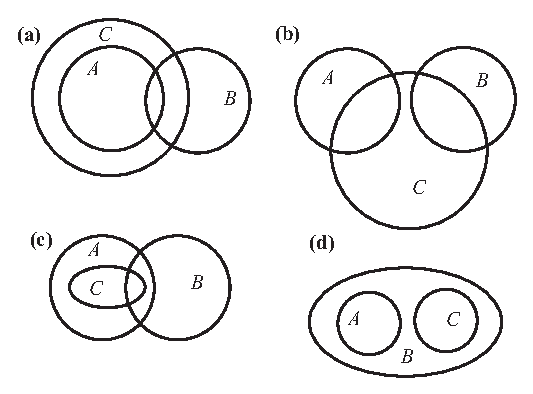
\includegraphics{xfig-exer12-41.eps}
\end{center}
\end{figure}


\item Using the standard setup for Venn diagrams with 3 sets,
\begin{enumerate}
\item $A \cap B$ corresponds to regions 2, 5.

\item $A \cap C$ corrresponds to regions 4, 5.

\item $(A \cap B) \cup (A \cap C)$ corresponds to regions 2, 4, 5.

\item $B \cup C$ corresponds to regions 2, 3, 4, 5, 6, 7.

\item $A \cap (B \cup C)$ corresponds to regions 2, 4, 5.

\item $(A \cap B) - C$ corresponds to region 2.
\end{enumerate}


\item \begin{enumerate}
\item Assume that $n$ is the sum of four consecutive integers.  So there exists an integer $k$ such that $n = (k - 1) + k + (k + 1) + (k + 2)$.  We then see that $n = 4k + 2$ and hence, 
$n \equiv 2 \pmod 4$.  Now assume that $n \equiv 2 \pmod 4$.  So there exists an integer $m$ such that $n = 4m + 2$.  We then see that $n = (m - 1) + m + (m + 1) + (m + 2)$ and hence, 
$n$ is the sum of four consecutive integers.

\item The set of all integers that are the sum of four consecutive integers is 
$\left\{ n \in \Z \mid n \equiv 2 \pmod 4 \right\}$.

\item The set of all natural numbers that are the sum of four consecutive integers is 
$\{10, 14, 18, 22, \ldots \, \}$.

\item Assume that $n$ is the sum of eight consecutive integers.  So there exists an integer $k$ such that
\[
n = (k - 3) + (k - 2) + (k - 1) + k + (k + 1) + (k + 2) + (k + 3) + (k + 4).
\]
We then see that $n = 8k + 4$ and hence, $n \equiv 4 \pmod 8$.  Now assume that 
$n \equiv 4 \pmod 8$.  So there exists an integer $m$ such that $n = 8m + 4$.  We then see that 
\[
n = (m - 3) + (m - 2) + (m - 1) + m + (m + 1) + (m + 2) + (m + 3) + (m + 4) 
\]
and hence, $n$ is the sum of eight consecutive integers.

\item The set of all integers that are the sum of eight consecutive integers is 
$\left\{ n \in \Z \mid n \equiv 4 \pmod 8 \right\}$.

\item The set of all natural numbers that are the sum of eight consecutive integers is 
$\{36, 44, 52, 60, \ldots \, \}$.
\end{enumerate}


\item This statement is false.  For a counterexample, we can use $U = \Z$ and let $A$ be the set of all odd integers and let $B$ be the set of all even integers.  In this case, 
$A \not\subseteq B$, $A \ne B$, and $B \not\subseteq A$.
\end{enumerate}




\subsection*{Explorations and Activities}
\setcounter{oldenumi}{\theenumi}
\begin{enumerate} \setcounter{enumi}{\theoldenumi}
\item \begin{enumerate}
\item The interval $\left( {a, b} \right)$  is a proper subset of   $\left( {a, b} \right]$ since 
$ b \in \left( a, b \right]$ and $b \notin \left( a, b \right)$.

\item The interval $\left[ a, b \right]$ is not a subset of $\left( a, + \infty \right)$ since 
$a \in \left[ a, b \right]$ and $a \notin \left( a + \infty \right)$.

\item $\left[ -3, 7 \right] \cap \left( 5, 9 \right] = \left( 5, 7 \right]$

\item $\left\{ {x \in \mathbb{R}} \mid \left| x \right| \leq 0.01 \right\} = \left[ -0.01, 0.01 \right]$

\item $\left\{  x \in \mathbb{R} \mid \left| x \right| > 2 \right\} = \left( { - \infty , 2} \right) \cup \left( {2, \infty } \right)$
\end{enumerate}


\item \begin{enumerate}
\item $[2, 5] \cap [-1, +\infty) = [2, 5]$ and $[2, 5] \cup [-1, +\infty] = [-1, +\infty)$

\item $[2, 5] \cap [3.4, +\infty) = [3.4, 5]$ and $[2, 5] \cup [3.4, +\infty) = [2, +\infty)$

\item $[2, 5] \cap [7, +\infty) = \emptyset$ and $[2, 5] \cup [7, +\infty)$ cannot be expressed as a single interval.

\item If $c \leq a$, then $[a, b] \cap [c, +\infty) = [a, b]$. If $a < c < b$, then 
$[a, b] \cap [c, +\infty) = [c, b]$.  If $c = b$, then $[a, b] \cap [c, +\infty) = {b}$.  If 
$b < c$, then $[a, b] \cap [c, +\infty) = \emptyset$.

\item If $c \leq a$, then $[a, b] \cup [c, +\infty) = [c, +\infty)$. If $a < c \leq b$, then 
$[a, b] \cup [c, +\infty) = [a, +\infty)$.  If $b < c$, then $[a, b] \cup [c, +\infty)$ cannot be expressed as a single interval.
\end{enumerate}



\item \setcounter{equation}{0}
\noindent
\textbf{Theorem~\ref{T:powerset}}.  Let  $n$  be a nonnegative integer and let  $A$  be a subset of some universal set.  If  $A$  is a finite set with  $n$  elements, then  $A$  has  $2^n $  subsets.  That is,  if  $\left| A \right| = n$, then  $\left| {\mathcal{P}\left( A \right)} \right| = 2^n $.

\vskip6pt
\noindent
For each nonnegative integer  $n$, let  $P\left( n \right)$ be, if  $A$  is a finite set with  
$n$  elements, then  $A$  has  $2^n $  subsets.

\begin{enumerate}
\item The statement  $P\left( 0 \right)$ is true since the empty set has  $2^0  = 1$ subset. 

\item The statement  $P\left( 1 \right)$ is true since a set with one element has  $2^1  = 2$ subsets.

The statement  $P\left( 2 \right)$ is true since a set with two elements has  $2^2  = 4$
 subsets. (The subsets of  $\left\{ {a, b} \right\}$ are  
$\emptyset$ , $\left\{ a \right\}, \left\{ b \right\}$, $\left\{ {a, b} \right\}$.)

\item Now assume that  $k$  is a nonnegative integer and assume that  $P\left( k \right)$ is true.  That is, assume that if a set has  $k$  elements, then that set has  $2^k $ subsets. 

Let  $A$  be a subset of the universal set with  $\left| A \right| = k + 1$, and let  $x \in A$.  Then, the set  $B = A - \left\{ x \right\}$  has  $k$  elements.  Since  $P\left( k \right)$
 is true, the set  $B$  has  $2^k $ subsets.

Now, by Lemma~\ref{L:inductivestepforsubsets},  each subset of  $A$  is a subset of  $B$  or a set of the form  
$C = B \cup \left\{ x \right\}$ where  $C$  is a subset of  $B$.  So, if  $B$  has  $2^k $
 subsets, then the number of subsets of  $A$ is equal to
\[
2^k  + 2^k  = 2 \cdot 2^k  = 2^{k + 1} .
\]
This proves that if  $P\left( k \right)$ is true, then  $P\left( {k + 1} \right)$ is true.  Hence, by the Second Principle of Mathematical Induction,  $P\left( n \right)$ is true for each nonnegative integer  $n$.
\end{enumerate}

\end{enumerate}





\hbreak
\endinput

\item 
\begin{enumerate}
\item 
\begin{figure}[h]
\includegraphics[2.5cm,1.8cm]{xfigexer-41-9a.bmp}
\end{figure}

\item 
\begin{figure}[h]
\includegraphics[2.5cm,1.8cm]{xfigexer-41-9b.bmp}
\end{figure}
